\documentclass[17pt, a1paper, portrait, margin=1cm, innermargin=0.5cm]{tikzposter}

% Polskie znaki i język (opcjonalnie, ale przydatne)
\usepackage[utf8]{inputenc}
\usepackage[T1]{fontenc}
% \usepackage[polish]{babel}

% Dodatkowe pakiety dla ozdobników i grafiki
\usepackage{graphicx}
\usepackage{amsmath, amssymb}
\usepackage{booktabs}
\usepackage{mwe}  % przykładowe obrazki (example-image)

\usepackage{twemojis}
\usepackage{transparent}
\usepackage{xcolor}
\usetikzlibrary{positioning}
\pgfdeclarelayer{background}
\pgfdeclarelayer{backgroundlayer}
\pgfsetlayers{background,backgroundlayer,main}
\usepackage[labelfont=bf]{caption}
\usepackage{tikzducks}
\usepackage{qrcode}
\usepackage{enumitem}

% --------------------------------------------------------------
% KOLORYSTYKA WŁASNA – nowoczesne, stonowane barwy
% --------------------------------------------------------------
\definecolor{myblue}{RGB}{0, 112, 192}       % głęboki błękit
\definecolor{mygray}{RGB}{240, 240, 240}     % jasnoszare tło bloków
\definecolor{myred}{RGB}{200, 60, 60}        % akcent (np. wyniki)
\definecolor{mygreen}{RGB}{60, 150, 80}      % akcent
\definecolor{almostwhite}{RGB}{243,236,226}
\definecolor{organiserblue}{HTML}{4C69AB}

% Ustawienie kolorów dla całego plakatu
\colorlet{titlebgcolor}{organiserblue!70!black}
\colorlet{titlefgcolor}{white}
\colorlet{blocktitlebgcolor}{organiserblue}
\colorlet{blocktitlefgcolor}{white}
\colorlet{blockbodybgcolor}{almostwhite}
\colorlet{blockbodyfgcolor}{black}
\colorlet{innerblocktitlebgcolor}{organiserblue!30}
\colorlet{innerblocktitlefgcolor}{black}
\colorlet{innerblockbodybgcolor}{white}

% --------------------------------------------------------------
% STYLE BLOKÓW – zaokrąglone rogi, delikatny cień
% --------------------------------------------------------------
\useblockstyle{Envelope}   % ładne, miękkie bloki
\usetitlestyle{Filled}     % tytuł wypełniony kolorem
\makeatletter
\setlength{\TP@blockverticalspace}{6mm}
\setlength{\TP@colspace}{8mm}
\setlength{\TP@titletoblockverticalspace}{0mm}
\makeatother


% --------------------------------------------------------------
% POCZĄTEK DOKUMENTU
% --------------------------------------------------------------

\makeatletter
\def\title#1{\gdef\@title{\scalebox{\TP@titletextscale}{%
\begin{minipage}[t]{\linewidth}
\centering
#1
\par
\vspace{0.5em}
\end{minipage}%
}}}
\makeatother %https://tex.stackexchange.com/a/180248

\title{\parbox{\linewidth}{\centering A Treatise on Shelling Bananas,\\{\LARGE or Why One Should Not Leave Antimatter in a Gravitational Field}}}
\author{Mateusz ,,{\textcolor{black}{$\blacksquare$}}'' Winiarski}
\institute{\large Faculty of Physics, Astronomy and Applied Computer Science, Jagiellonian University in Kraków, Poland}

\newcommand{\SeMPowisko}{%
\large S\normalsize%
\kern-.3em \lower.2ex\hbox{e}%
\lower.2ex\hbox{\large M\normalsize}%
\kern-.1em \raise.1ex\hbox{\large P\normalsize}%
\kern-.3em \lower.2ex\hbox{o}%
\kern-.2em \raise.2ex\hbox{w}%
\lower.2ex\hbox{i}%
s%
\raise.2ex\hbox{k}%
\kern-.3em \lower.2ex\hbox{o}%
}

\begin{document}

\maketitle

\node[below left=1.5cm and 1.5cm] at (topright){
{\transparent{0.5}\twemoji[width=7cm]{magnet}}
} ;

\coordinate (topleft)     at (topright -| bottomleft); %https://tex.stackexchange.com/a/505515
\node[below right=1.5cm and 1.5cm] at (topleft){
{\transparent{0.5}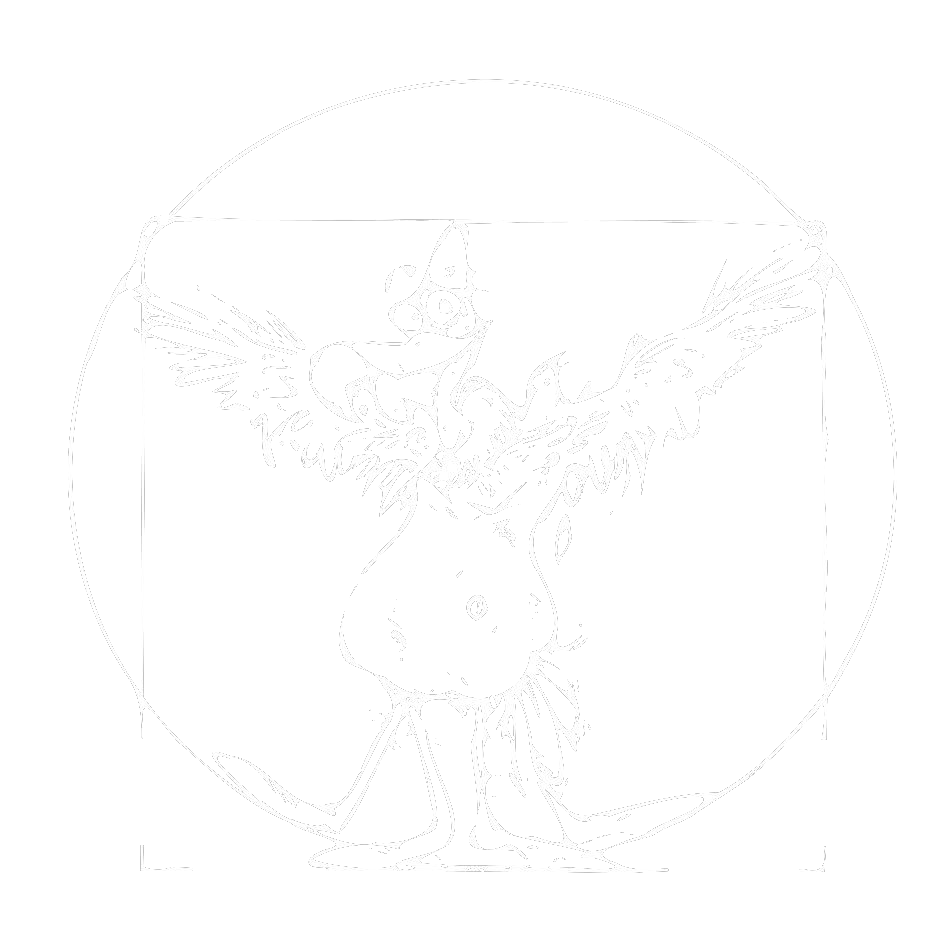
\includegraphics[width=7cm]{janusz.png}}
} ;

\begin{scope}[on background layer]
\node[yshift=1.5cm,xshift=-2cm,opacity=0.1] at (current page.south east)
      {
      
\includegraphics[scale=0.4, angle=25]{ptaki.pdf}
      };
\end{scope}


% --------------------------------------------------------------
% BLOK STRESZCZENIA (pełna szerokość)
% --------------------------------------------------------------
\block{Abstract}{%
Does antimatter interact with gravitational field the same way as matter? While ALPHA-g confirmed
this for antihydrogen, a purely leptonic system – positronium – remains a compelling target. This
poster explores how metastable $2^3S$ Ps beams and matter-wave interferometry can probe gravitational
acceleration on antimatter, and why it does not work.

}

\block{Introduc(k)tion\hspace{0.5cm} \protect\raisebox{-0.15em}{\tikz[scale=0.5]{\duck[body=yellow!85!orange,bill=orange,jacket=black, strawhat=brown!50!black, ribbon=gray, bowtie=organiserblue!70!black]}}}{%
        \begin{minipage}[t]{0.58\linewidth}
            Antiparticles are "mirror counterparts" of regular particles: according to CPT (charge-parity-time) parity they can be thought of as particles of reversed charge and parity, or going backward in time.

            Antimatter particles in contact with matter partners annihilate into gamma rays, according to mass-energy equivalence ($E=m$). Positrons from beta-plus decays can form electron-positron bound state (\emph{positronium}) before decaying, which acts like an exotic atom and decays with an average lifetime of 124 ps ($1^1S$), 142 ns ($1^3S$), 1.14 $\mu$s ($2^3S$)...

            Three common ways of antimatter production are: 1) high-energy particle collisions in synchrotron accelerators -- protons collide with metallic targets and their kinetic energy is high enough to create proton-antiproton pair; 2) beta-plus decay -- proton transforms into neutron in a neutron-deficient nucleus (like $^{11}C,\ ^{15}O,\ ^{18}F$...), producing a positron; 3) cosmic-ray interactions.

            The main problem of antimatter is its containment (as you have probably seen in 2009 film \mbox{\emph{Angels~\&~Demons}}).
        \end{minipage}\hfill
        \begin{minipage}[t]{0.41\linewidth}
            \vspace{0pt}
            \centering
            \begin{minipage}[t]{0.24\linewidth}
                \centering
                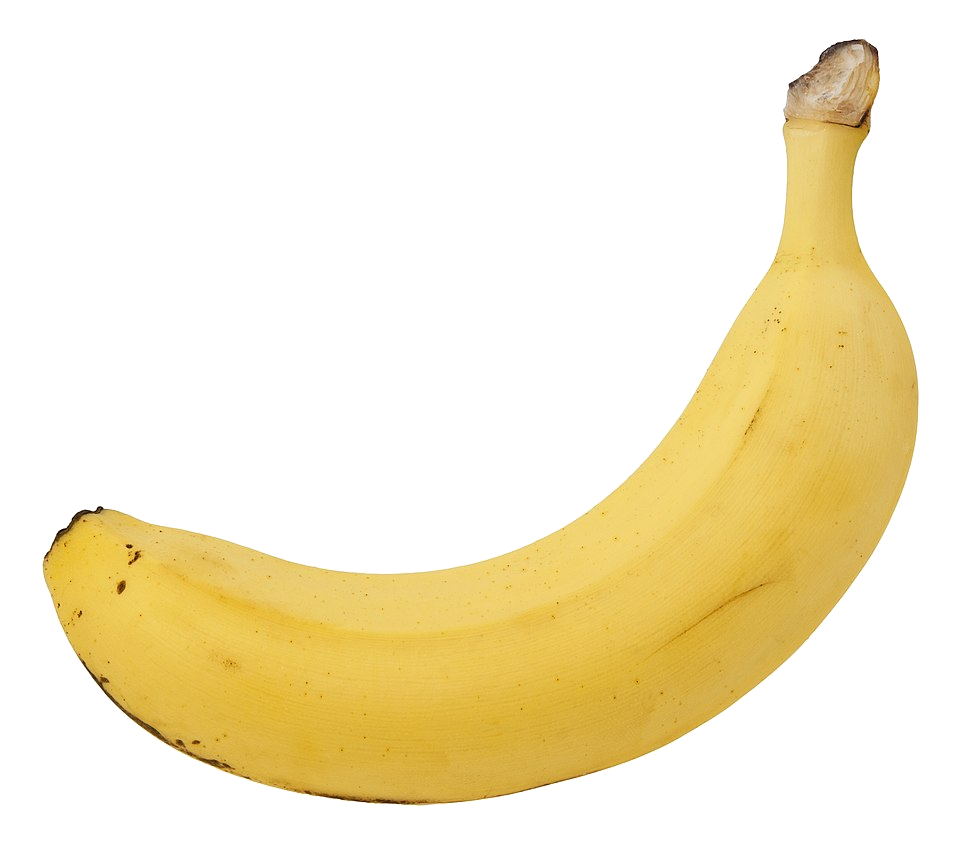
\includegraphics[width=\linewidth]{sword.png}
                \captionof{figure}{\scriptsize A regular banana undergoes $\sim$15 decays of K-40 per second; only a tiny fraction of these ($\sim$0.001\%) are positrons.}
            \end{minipage}\hfill
            \begin{minipage}[t]{0.24\linewidth}
                \centering
                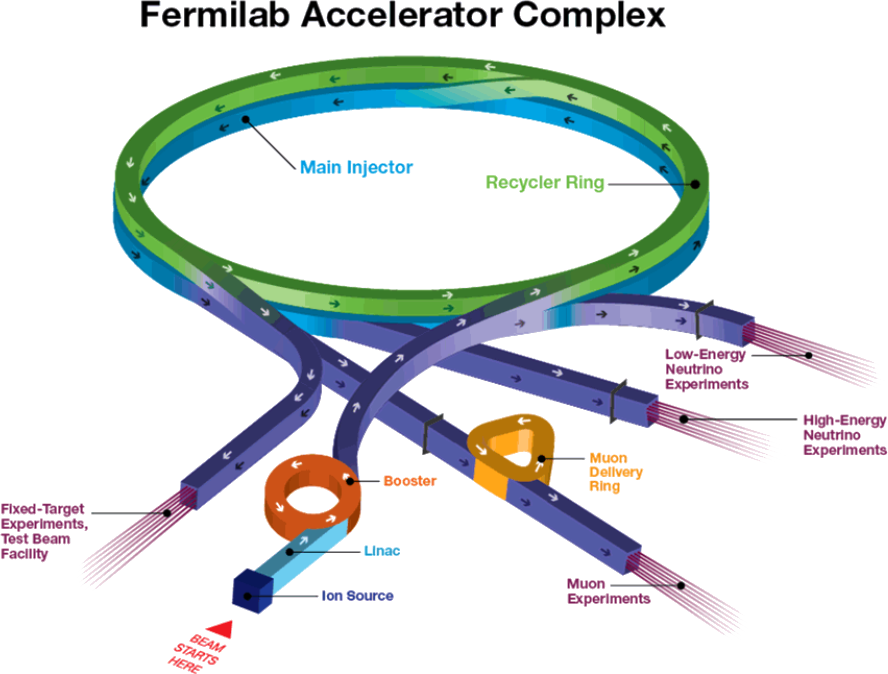
\includegraphics[width=\linewidth]{fermi.png}
                \captionof{figure}{\scriptsize In a particle collider, a centre-of-mass energy of $\sim$1.88~GeV is sufficient to create a proton–antiproton pair. Fixed-target production (as used at Fermilab’s Antiproton Source, which used to be world's greatest antimatter producer) requires a proton beam of kinetic energy $\sim$5.6~GeV. }
            \end{minipage}\hfill
            \begin{minipage}[t]{0.24\linewidth}
                \centering
                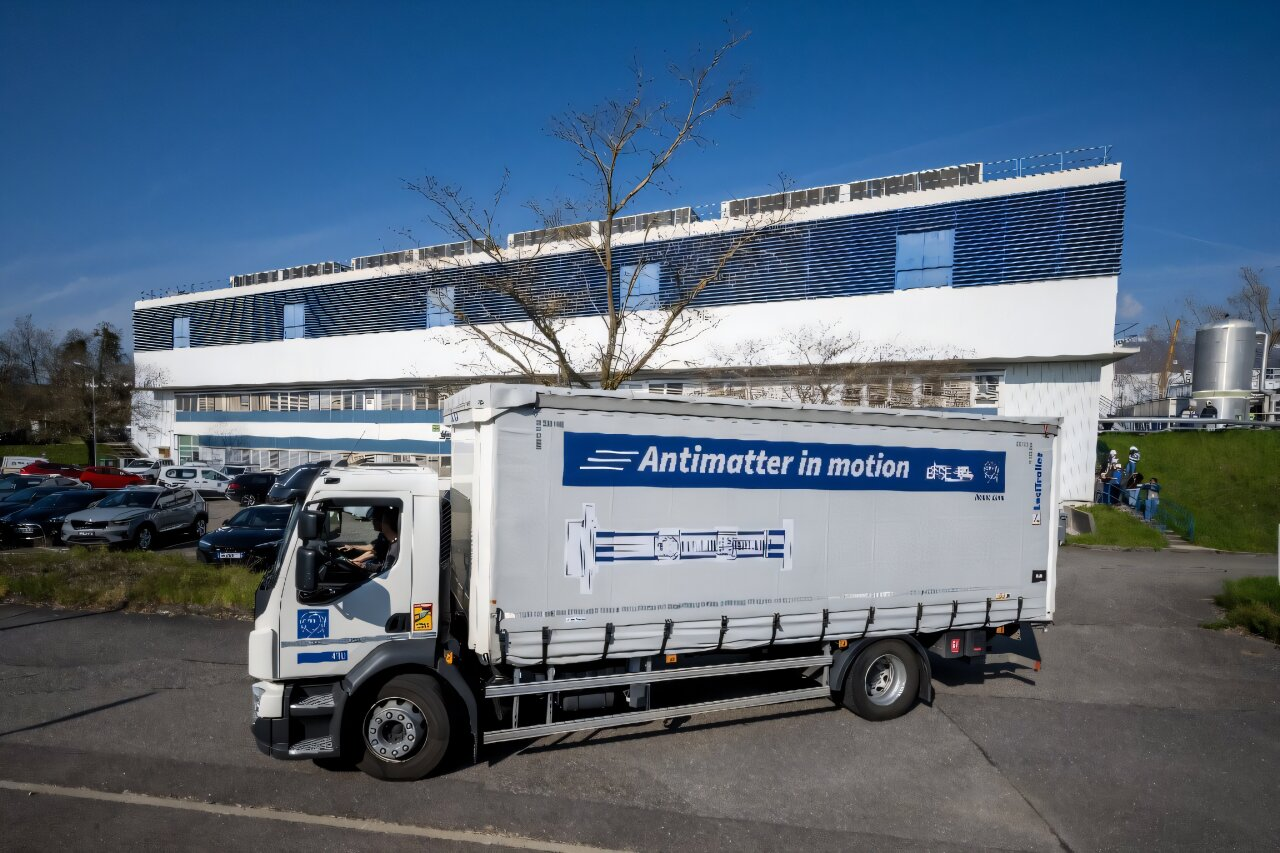
\includegraphics[width=\linewidth]{lorry.png}
                \captionof{figure}{\scriptsize After deceleration, you can store antimatter in magnetic traps; and since March 2026, you can even transport it in truck (as shown by BASE experiment)}
            \end{minipage}
            \begin{minipage}[t]{0.24\linewidth}
                \centering
                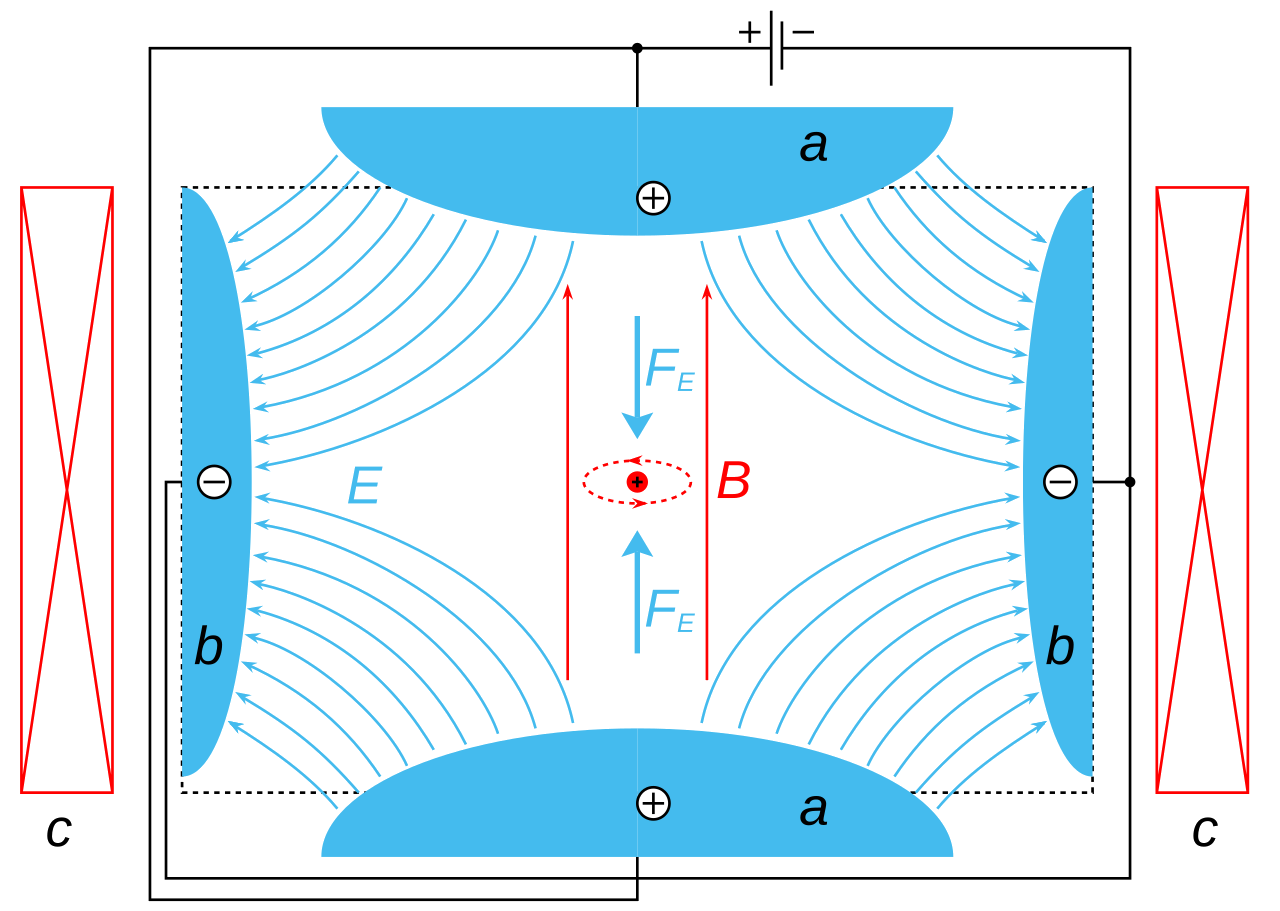
\includegraphics[width=\linewidth]{penning.png}
                \captionof{figure}{\scriptsize Schematic view of Penning trap with electric (blue) and magnetic (red) field indicated, generated by electrodes and coils respectively}
            \end{minipage}
        \end{minipage}
    }

\block{}{
% \begin{figure}
    \centering
    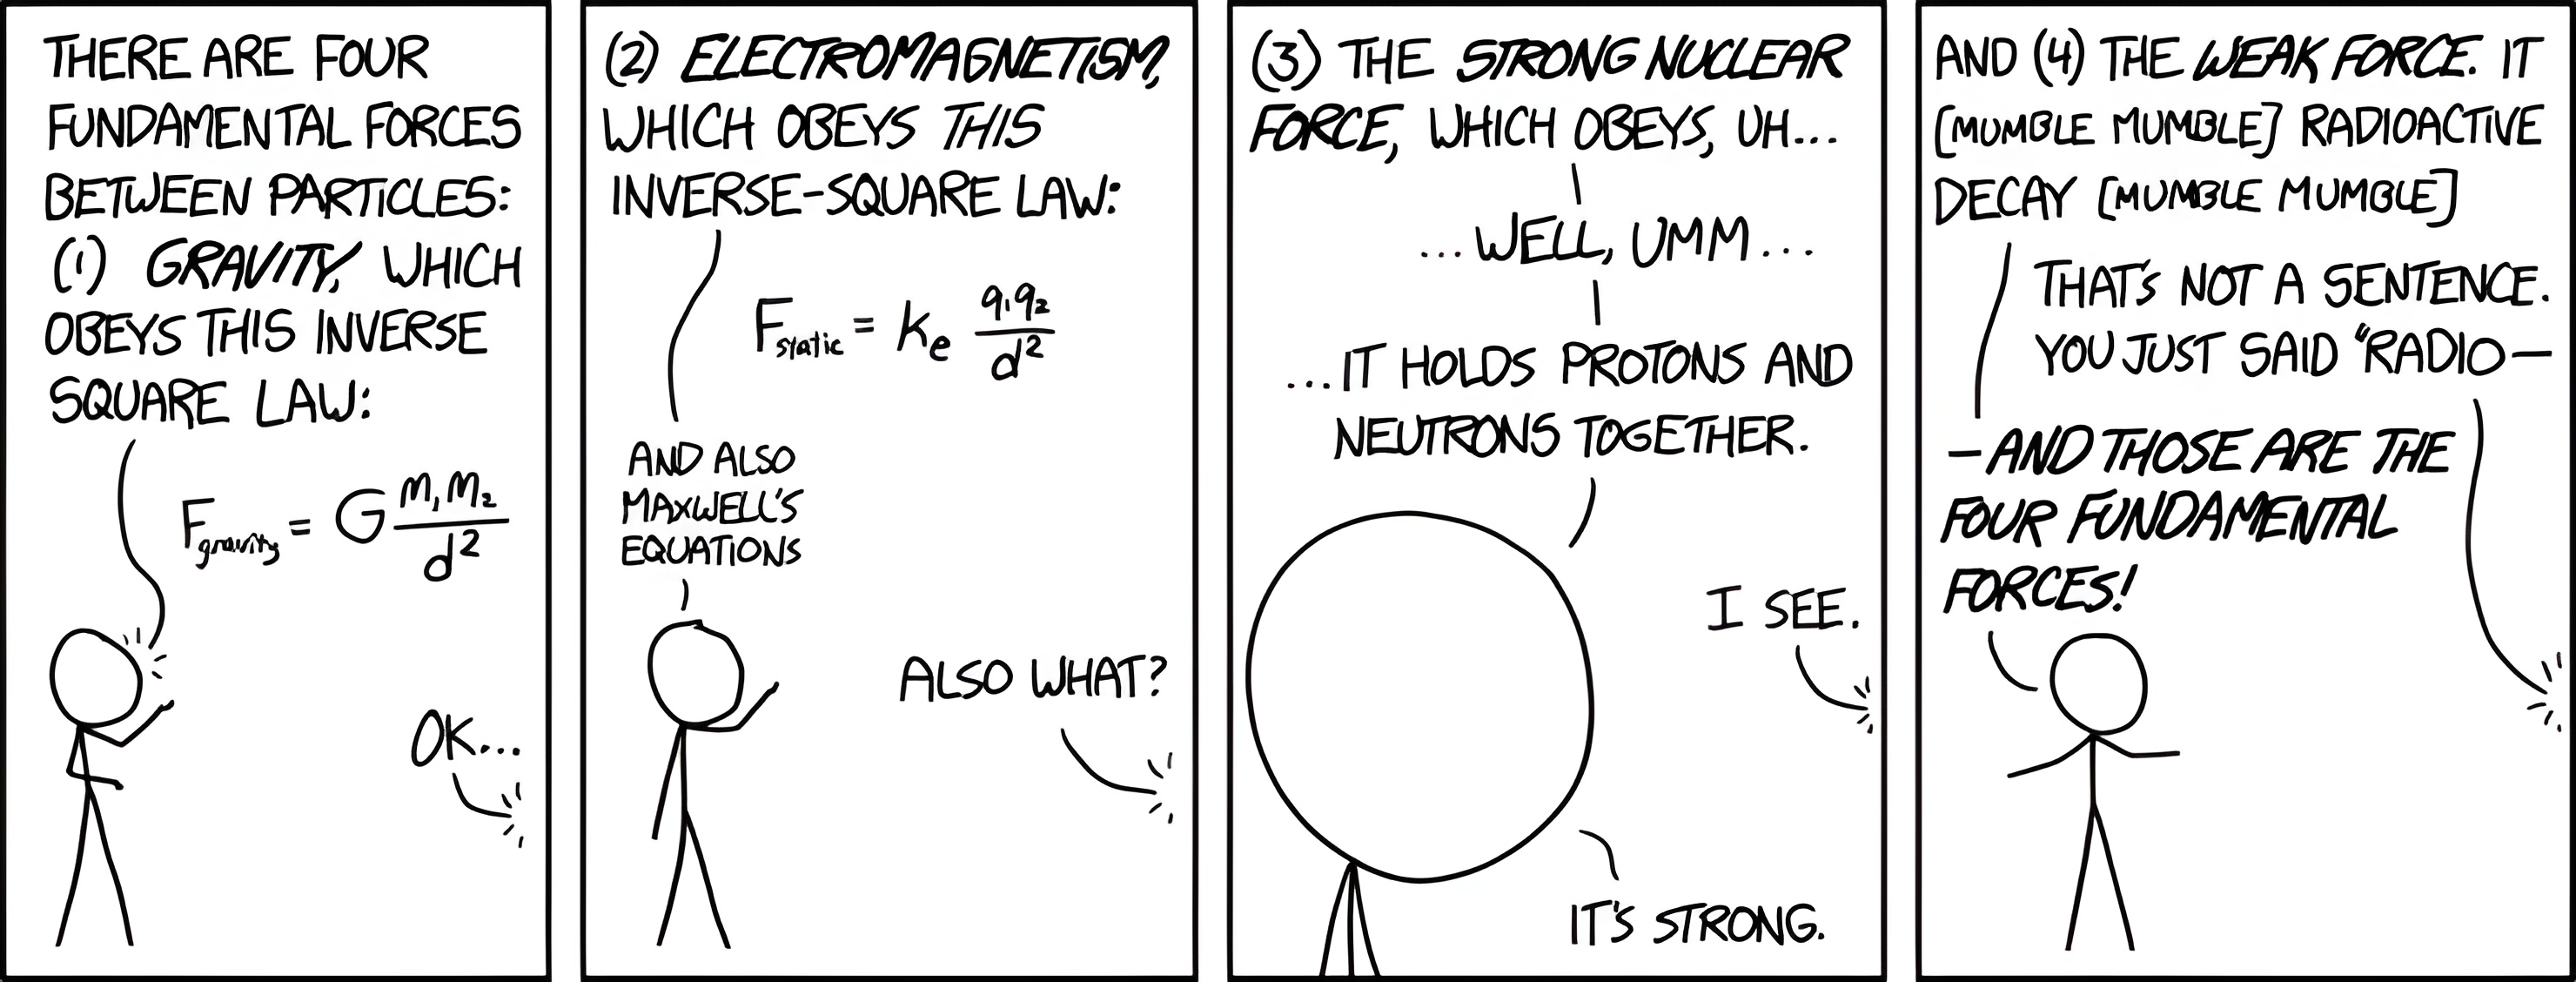
\includegraphics[width=0.75\linewidth]{1489.png}
    \captionof{figure}{"Of these four forces, there's one we don't really understand." "Is it the weak force or the strong--" "It's gravity."}
    % \caption{Enter Caption}
    % \label{fig:enter-label}
% \end{figure}
}

% --------------------------------------------------------------
% UKŁAD KOLUMNOWY (dwie kolumny)
% --------------------------------------------------------------
\begin{columns}
    \column{0.27}
    \block{Theory}{%
        In theory, according to several simple arguments, antimatter should fall just like ordinary matter.

        \vspace{4mm}

        \begin{itemize}[leftmargin=0cm,itemsep=0.35em,parsep=0pt,topsep=0.3em]
        %   \setlength{\itemindent}{0em}
            \item \textbf{CPT% {\rm(charge+parity+time)}
            \ symmetry:} according to the CPT theorem, antimatter should experience the same gravitational acceleration as matter
            \item \textbf{photon behaviour:} photons are their own antiparticles, and they act just like General Relativity laws tell them so
            \item \textbf{conservation of energy:} if antimatter goes up, we can annihilate it "higher" than it was produced
        \end{itemize}

        However...
        \begin{itemize}[leftmargin=0cm,itemsep=0.35em,parsep=0pt,topsep=0.3em]
            \item \textbf{Kowitt theory:} antiparticles are "holes" in Dirac particle sea with negative gravitational mass
            \item \textbf{Santilli-Villata theory:} antimatter exists in inverted space-time, which is projected to our reality as negative motion
            \item \textbf{Cabbolet's theory:} particles move in "stepwise" motion, alternating between state of rest and "wave--like" movement
            \item \textbf{dark matter???}%
        \end{itemize}
        \vspace{-0.4cm}%
    }

    \column{0.27}
    \block{Antihydrogen ($p^-e^+$)}{%
        ALPHA {\footnotesize(Antihydrogen Laser Physics Apparatus)} experiment in CERN has shown that...
%
        \begin{tikzfigure}
        \centering
        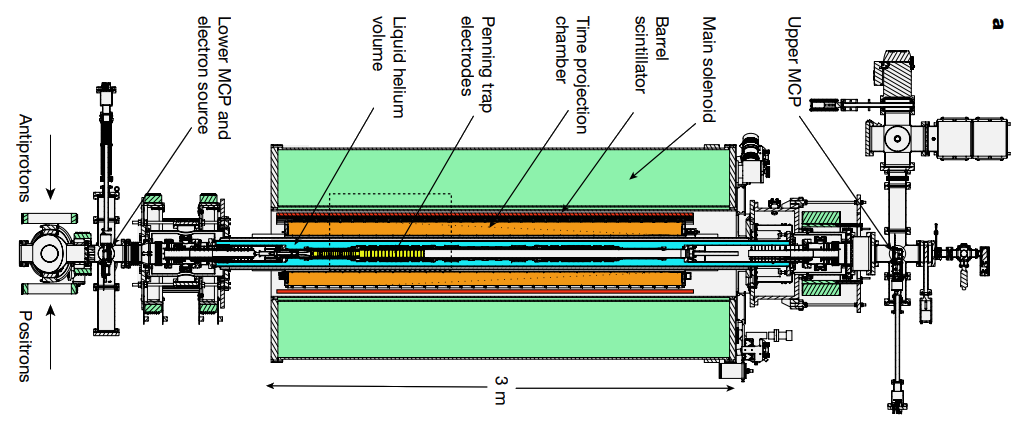
\includegraphics[width=0.9\linewidth]{alpha1.png}
        \end{tikzfigure}
%
        ...we decelerate antihydrogen and put it in Penning magnetic traps, then slowly ramp down current and observe, with and without magnetic bias, where particles annihilate...
        {
            \begin{tikzfigure}
        \centering
        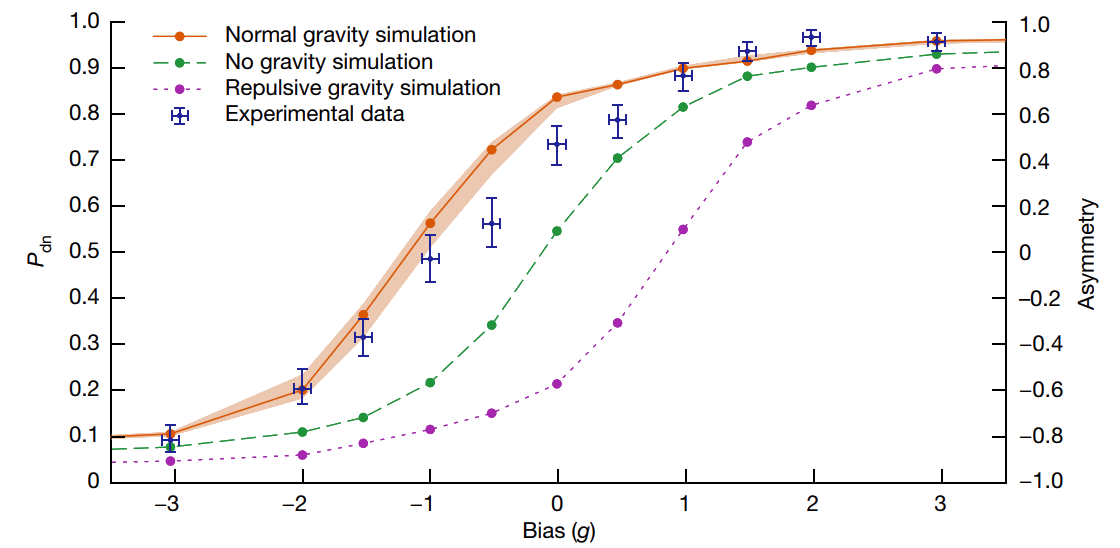
\includegraphics[width=0.8\linewidth]{alpha5.png}
        \end{tikzfigure}
        }
        \raggedright%
%
        ...the observed local gravitational acceleration of antihydrogen atoms is $a_{\bar{g}} = (0.75 \pm 0.13 \text{ (stat. + syst.)} \pm 0.16 \text{ (sim.)}) g$.
    }

    \column{0.27}
    \block{Positronium ($e^-e^+$)}{%
    Recent proposals show that...%
    \begin{tikzfigure}
    \centering
    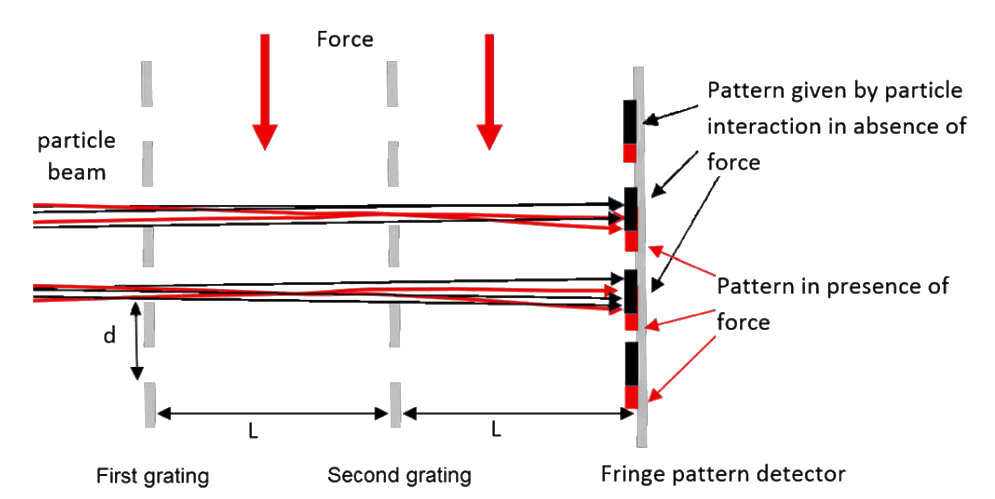
\includegraphics[width=0.7\linewidth]{interf.png}
    \end{tikzfigure}%
%
    using a simple deflectometer we can measure the curvature of the motion path of neutral positronium systems.

    Unfortunately...%
    \vspace{-0.35cm}
    \begin{tikzfigure}%
    \centering%
    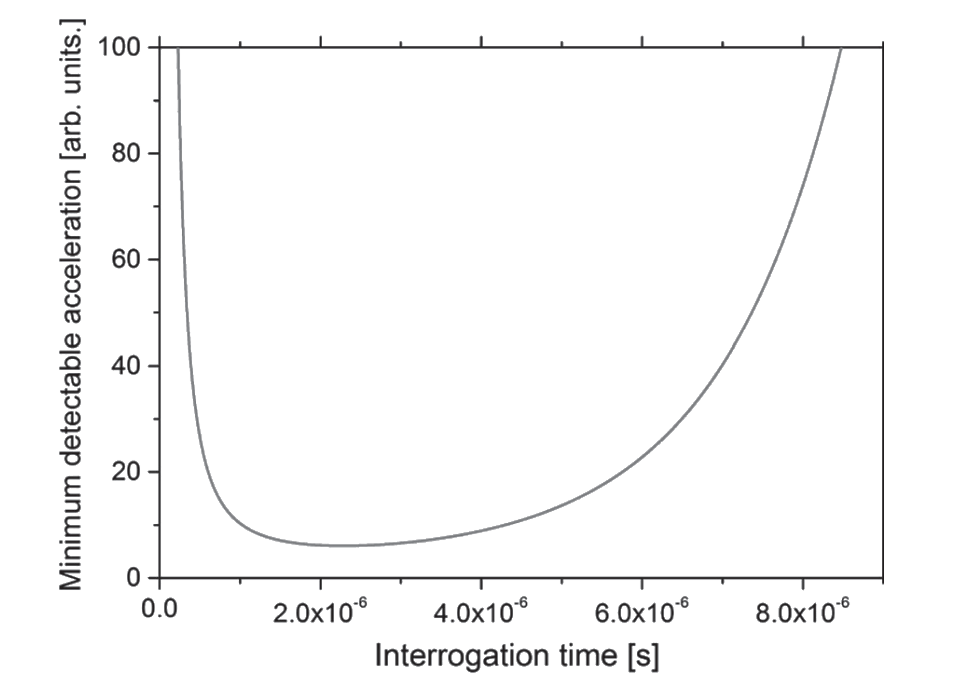
\includegraphics[width=0.5\linewidth]{sensi.png} %
    \end{tikzfigure}%
    \vspace{-0.35cm}

%
    using current technology measurement of Earth gravitational acceleration would take $\sim$5 years.

    Solution: laser collimation, Raman excitation scheme

        \raggedleft $\to$ \emph{to be continued}

        \vspace{0.3cm}

    }

    \column{0.19}
    \block{References}{%

        \centering

    \qrcode[height=4cm]{http://tiny.cc/postermw}\\\vspace{2mm}
    {\footnotesize\texttt{http://tiny.cc/postermw}}
    }
    \vspace{1cm}
    \block{}{%
        \hspace{-0.025\linewidth}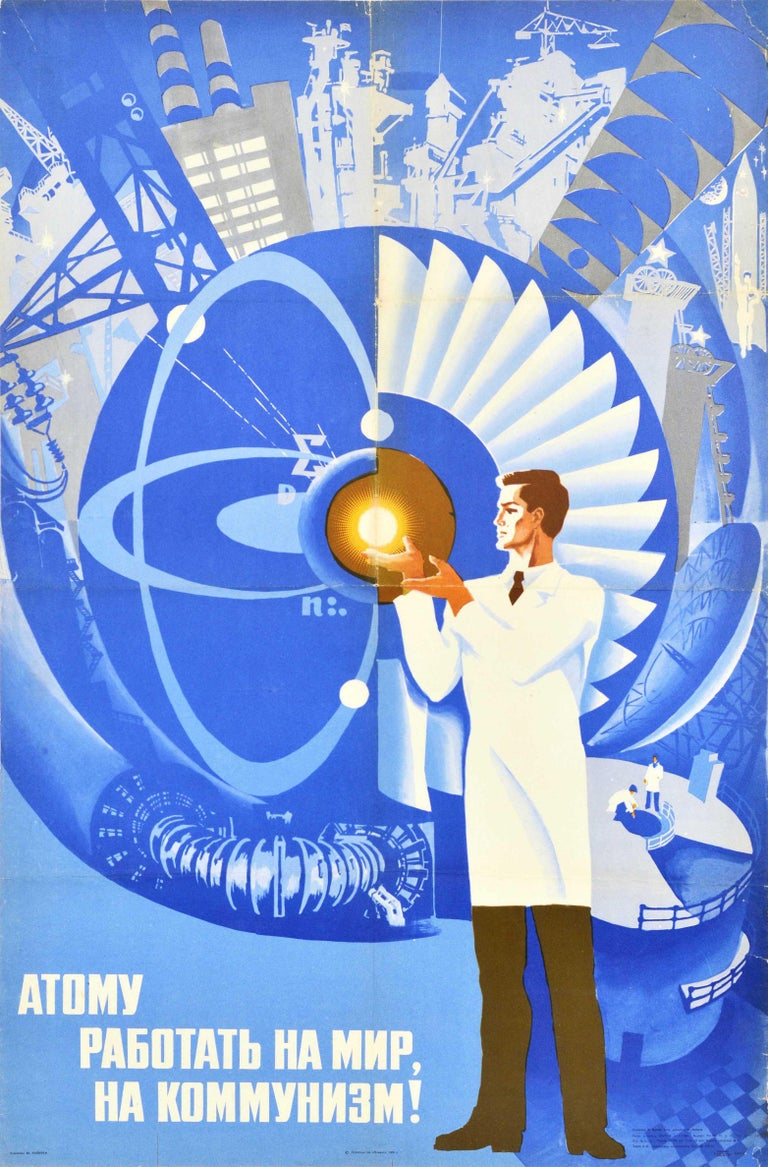
\includegraphics[width=1.05\linewidth]{atomy.png}%

    }
\end{columns}

% Opcjonalna stopka z datą i miejscem
\node[above right=0cm and 0cm] at (bottomleft) {24th \SeMPowisko{}, April 23rd-26th 2026};
\end{document}